\chapter{Background} \label{background}

Skylab is built using Ruby on Rails, a well-known web development framework with a great support from a large community, used widely in the industries by companies like Twitter, Groupon, Bloomberg, Airbnb and many more\cite{citation1}. There are many reasons why we have chosen Ruby on Rails. Firstly, Ruby is clean, elegant and easy to read and readability and elegance of Ruby enables programmers to be more productive. Secondly, Ruby on Rails is adopting many advanced industrial conventions and this enables contributors to have good exposure to programming in the industry. What is more, scaffolding and many gems in Ruby community can significantly simplify programmers` work by saving time and effort in ``reinventing the wheels''. And the popularity and activeness in Ruby on Rails` community ensures that getting continuous support would be easy and many resources can also be available online. Last but not least, Ruby on Rails community has a favor for open source contribution which aligns well with the open source nature of Skylab.

For the selection of database, we used PostgreSQL. Part of the reason is that it is open source and quite mature, with good drivers available in many languages\cite{citation2}. Besides, we need full ACID(atomicity, consistency, isolation and durability) compliance for consistency of data and we do not need scalability to multiple servers in the foreseeable future\cite{citationACID}. And PostgreSQL has recently added implementation for rich data structures such as JSON which would make development much easier\cite{citation3}.

Puma is the web server we have chosen for Skylab. Among common Ruby web servers such as Passenger, Unicorn, Rainbows! and Puma, Puma is considered to be fast and memory friendly according to online benchmarking\cite{citation4}. Puma is built for high-concurrency and speed and more and more developers to switching to Puma in Rails community\cite{citation5}.

We have selected Nginx as our HTTP server. Nginx has grown in popularity since its release due to its light-weight resource utilization and its ability to scale easily with low memory usage. It excels at serving static content quickly and is designed to pass dynamic requests off to other software that is better suited for those purposes\cite{citation6}. There are also some benchmarking results that indicate the superiority in Nginx handling concurrent access and low memory usage of Nginx\cite{citation7}.

A high-level overview of the architecture of Skylab is illustrated in Figure~\ref{fig:Skylabarch}. Incoming requests to server will first be forwarded to Puma worker processes by Nginx. After that the corresponding Skylab code in Ruby on Rails framework will be executed and when accessing database is required, PostgreSQL will come into picture and serve the data.

\begin{figure}[h]
  \centering
  \includegraphics[width=0.9\textwidth]{Images/Skylab_Arch.png}
  \caption{Architecture of Skylab}
  \label{fig:Skylabarch}
\end{figure}

\section{System design}

\subsection{MVC pattern in Ruby on Rails}

The basic MVC structure of Rails is shown in Figure~\ref{fig:RailsMVC}:

\begin{figure}[h]
  \centering
  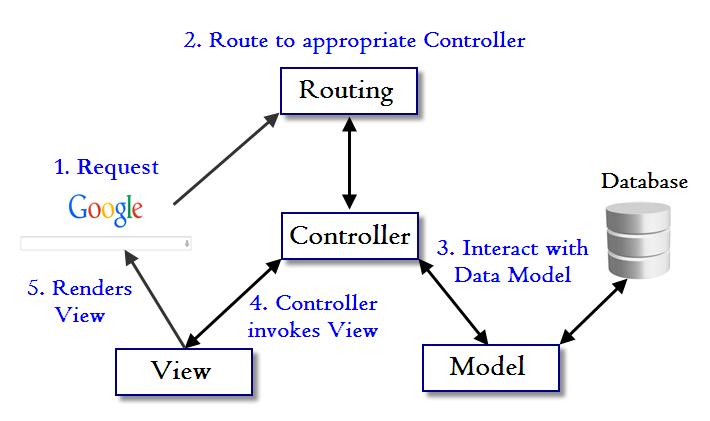
\includegraphics[width=0.85\textwidth]{Images/Rails_MVC.png}
  \caption{Illustration of how MCV works in Rails. Excerpted from \cite{citationMVC}}
  \label{fig:RailsMVC}
\end{figure}

After request is received by Ruby on Rails framework, the router will look at the pattern of the requested URL path and send it to the corresponding method of the target controller class. The controller is supposed to query models and gather necessary information for rendering the view. Last but not least, the response will be sent back to user for viewing.

So the most fundamental component in this whole process is model, which stores all the business data. A good design of model can in fact save a lot of trouble when it comes to writing controllers.

\subsection{Overview of Models in Skylab}

An overview of current models` design would be as Figure~\ref{fig:SkylabER}(source available at \cite{citationERSource}).

\begin{figure}[h]
  \centering
  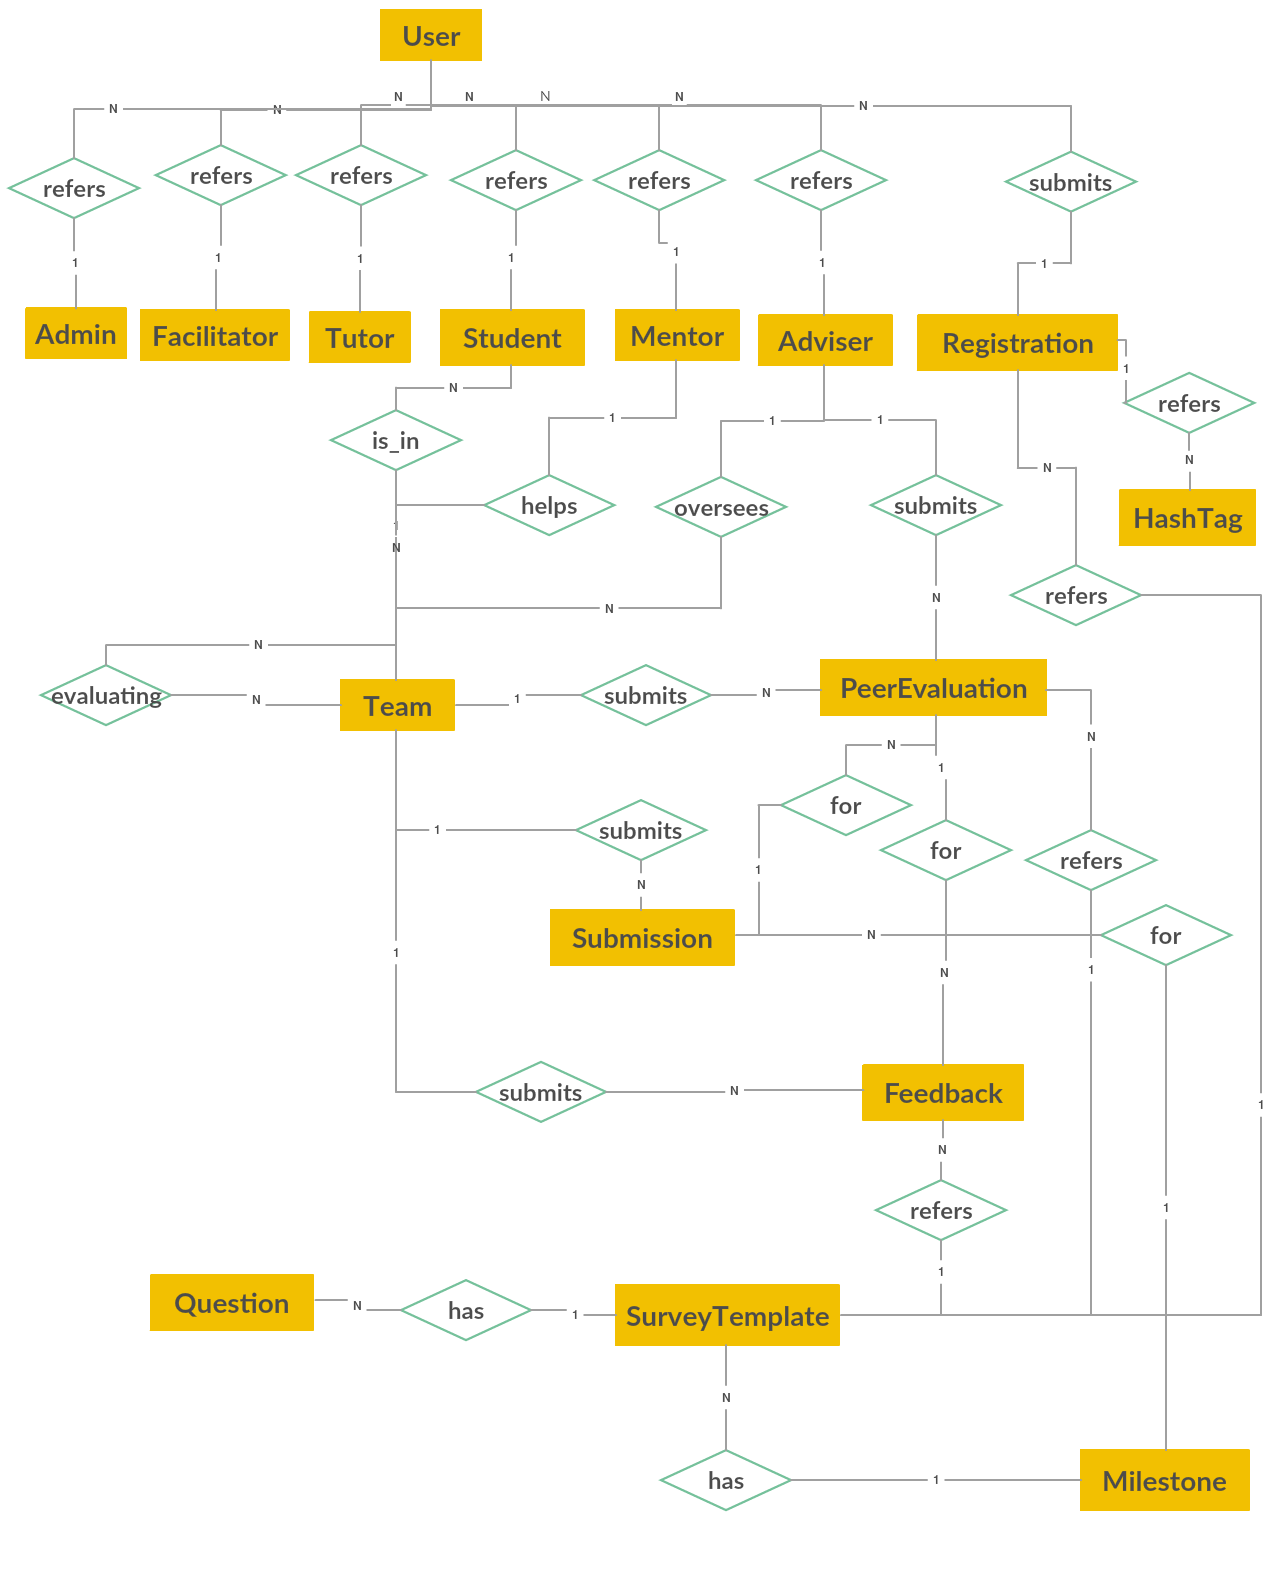
\includegraphics[width=\textwidth]{Images/Skylab_ER.png}
  \caption{Current ER diagram for Skylab}
  \label{fig:SkylabER}
\end{figure}

As you can see from the entity relation diagram shown in Figure~\ref{fig:SkylabER}, users' basic information is captured in the \textit{User} model and each user may have different roles such as \textit{Admin}, \textit{Student}, \textit{Adviser}, \textit{Mentor}, \textit{Tutor} and \textit{Facilitator}. Each user can have only one of any role in a cohort —-- meaning that if \textit{User} A is an \textit{Adviser} B for cohort 2015, then he/she's adviser role for cohort 2015 will only be B. But for cohort 2016 if \textit{User} A is an adviser again, then it is another \textit{Adviser} role C. Roles like \textit{Facilitator}, \textit{Tutor} do not have practical meanings in the system but only for display in public staff page. \textit{Admin} is supposed to overlook manage everything in Skylab. The remaining roles, \textit{Adviser}, \textit{Mentors} and \textit{Student} are connected via different relationships.

Each student has a \textit{Team} and a team has an \textit{Adviser} and a \textit{Mentor}(optional, only if the team requested). A group of teams under the same adviser is called an \textit{Evaluation Group} and evaluating relationships will be assigned from team to team in the same \textit{Evaluation Group}. Each team will create \textit{Submissions} to \textit{Milestones} to report their progress and their adviser and assigned evaluator teams will submit \textit{PeerEvaluations} to the team`s \textit{Submissions}. A \textit{SurveyTemplate} contains \textit{Questions} for a \textit{Feedback}, which is for evaluated team to provide feedback to their evaluator teams. After receiving the \textit{PeerEvaluation}, the team is supposed to submit \textit{Feedback} to rate the helpness of received \textit{PeerEvaluations}.

Before Orbital officially starts, interested students need to register in Skylab first. A \textit{Registration} will be created to record information about the student and his/her interested topics of project in the summer for recommending potential teammates if they do not have a partner in mind at the time of registration. \textit{Registration}, \textit{PeerEvaluation} and \textit{Feedback} will all make references to a \textit{SurveyTemplate}, which contains some \textit{Questions} to be answered.

\subsection{Overview of Controllers in Skylab}

Controllers will query models to get information needed to present views or make modifications to models if requested. Therefore they are crucial in powering a Rails application and in Skylab we have well-defined controllers to carry out different tasks. A class digram of all controllers in Skylab is shown in Figure~\ref{fig:SkylabControllers}.

\begin{figure}[h]
  \centering
  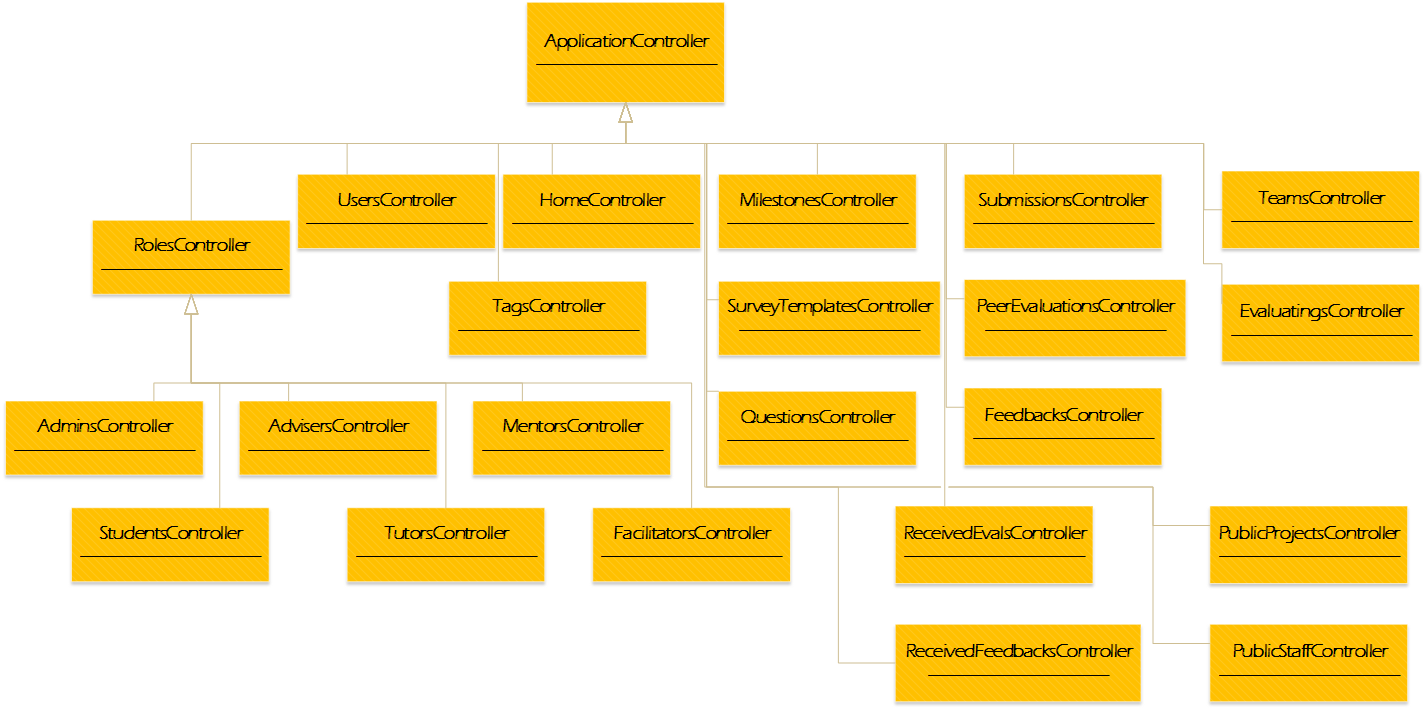
\includegraphics[width=\textwidth]{Images/Skylab_Controllers.png}
  \caption{Current Class diagram of controllers in Skylab}
  \label{fig:SkylabControllers}
\end{figure}

ApplicationController is the base of all other controllers. Utility methods such as access control, page title and handling of exceptions are included in ApplicationController and it also includes auxiliary modules such as CohortHelper to enrich its functionality. RolesController is the base class of all roles` controller classes: AdminsController, AdvisersController, MentorsController, StudentsController, FacilitatorsController and TutorsController. These roles share quite a lot in common so they will share request processing methods and they will override data related methods or provide some handlers for special cases. Other controllers are as follows:

\begin{itemize}
  \item \textbf{HomeController}: serves home page to user only.
  \item \textbf{UsersController}: manages listing, creation, editing and display of users and also includes functionality for admin to masquerade as any user, for new users to register as students in Orbital.
  \item \textbf{TagsController}: lists tags based on specified filters.
  \item \textbf{MilestonesController}: handles listing, creation, editing and display of milestones.
  \item \textbf{SurveyTemplatesController}: handles listing, creation, editing and display of survey templates and also serves as interface for editing of questions belonging to current survey templates. 
  \item \textbf{QuestionsController}: manages Ajax requests to create, edit or delete a question.
  \item \textbf{SubmissionsController}: manages creation, editing and display of submissions by students.
  \item \textbf{PeerEvaluationsController}: handles creation, editing and display of peer evaluations from evaluator teams or advisers to evaluated teams.
  \item \textbf{FeedbacksController}: manages creation, editing and display of feedback from evaluated team to evaluator teams or advisers.
  \item \textbf{ReceivedEvalsController}: compiles a set of received peer evaluations for a team in one milestone.
  \item \textbf{ReceivedFeedbacksConroller}: compiles a set of received feedback for a team or an adviser in one milestone.
  \item \textbf{PublicProjectsController}: serves completed teams` projects to the public.
  \item \textbf{PublicStaffController}: serves staff of Orbital program to the public.
  \item \textbf{TeamsController}: manages listing, creation, editing and display of teams.
  \item \textbf{EvaluatingsController}: handles listing, creation, editing and display of evaluating relation among teams.
\end{itemize}

Controller manages a collection of \textit{resources} in Skylab, meaning that each controller is managing(list, create, edit and display) usually one model class only for higher cohesion. If dependency on other models is needed, for example, SurveyTemplate will manage questions belonging to current SurveyTemplate, the requests will be handled by Ajax requests to separate concerns.

Skylab is following Ruby on Rails convention for controller classes. A basic controller that manages a collection would have the following structure illustrated in Figure~\ref{fig:SkylabSampleController}.

\begin{figure}[h]
  \centering
  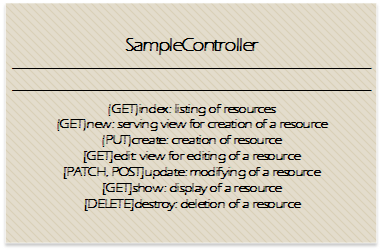
\includegraphics[width=0.5\textwidth]{Images/Skylab_Sample_Controller.png}
  \caption{Sample controller class in Skylab}
  \label{fig:SkylabSampleController}
\end{figure}

These methods —-- index, new, create, edit, update, show and destroy —-- have included all the basic actions to be done with a collection of resources. Following such a convention would not only make controller class in Skylab consistent and easy to read, but also align well with a more human-readable RESTful URL design.

\section{Development process}

As Skylab is a web application for which version does not mean anything in particular, we have adopted GitHub flow in our development process\cite{citation8}. So the master branch always contains the latest stable and deployable code base. Each feature will be developed on a feature branch and once the feature is ready, a pull request is created against master. After code review and all tests passes, pull requests will be merged into master and ready for deployment. Figure~\ref{fig:GithubFlow} illustrates the process as well.

\begin{figure}[h]
  \centering
  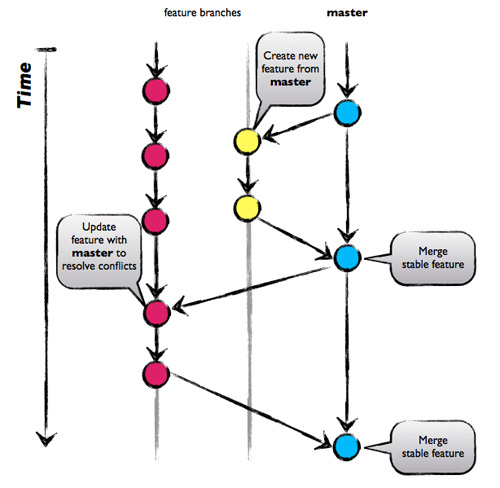
\includegraphics[width=0.85\textwidth]{Images/Github_Flow_Branching_Model.png}
  \caption{Branching diagram for GitHub Flow. Excerpted from \cite{citation8}}
  \label{fig:GithubFlow}
\end{figure}

By using GitHub flow and services such as Travis as the continuous integration service, CodeClimate as the code quality monitoring service, we can keep the development of Skylab agile and fast. Besides GitHub flow has enabled Skylab to deployed regularly, which is essential for timely improvement of user experience\cite{citation9}.
